%% ------------------------------------------------------------------- %%
%% ------------------------------------------------------------------- %%
%% ------------------------------------------------------------------- %%
%% ------------------------------------------------------------------- %%
\chapter{Experimentos}
\label{cap:experimentos}

\lhead{\emph{Experimentos}} 

%% ------------------------------------------------------------------- %%
%% ------------------------------------------------------------------- %%
%% ------------------------------------------------------------------- %%
%% ------------------------------------------------------------------- %%
%% ------------------------------------------------------------------- %%
%% ------------------------------------------------------------------- %%

%% -------------------------------------------------------------------- %%
%% -------------------------------------------------------------------- %%

En este capítulo, detallamos la metodología utilizada para los experimentos. Esta metodología  involucró utilizar la base de datos Anthem \citep{mei2021anthem} para entrenar los modelos, se comparó los modelos TAPE, ESM2 y ProtBert-BFD despues de aplicar \textit{fine-tuning}. Adicionalmente, se comparó el desempeño de estos al aplicar \textit{Gradient Accumulation Steps} (GAS)  y una metodología de congelación de capas. Finalmente, se comparó estos modelos con herramientas del estado del arte: NetMHCpan4.1 \citep{reynisson2020netmhcpan} y MHCFlurry2.0 \citep{o2020mhcflurry}, Anthem \citep{mei2021anthem}, Acme \citep{hu2019acme} y MixMHCpred2.2 \citep{gfeller2023improved}.

\section{Modelos BERT}

Como se detalló en el Capítulo \ref{cap:propuesta}, los modelos BERT pre-entrenados para realizar \textit{fine-tuning} fueron: TAPE \citep{rao2019evaluating}, ProtBert-BFD \citep{elnaggar2021prottrans} y ESM2 (ESM2(t6), ESM2(t12), ESM2(t30), ESM2(t33)) \citep{lin2023evolutionary}. Tanto ProtBert como ESM2 constituyen una familia de varios modelos; sin embargo, para esta tesis se escogió ProtBert-BFD de la familia de modelos ProtBert, y ESM2(t6), ESM2(t12), ESM2(t30), ESM2(t33) de la familia de modelos ESM2. Todos estos modelos se basan en una red \textit{Transformer} BERT que ha sido pre-entrenada con grandes volúmenes de secuencias de proteínas. En la Tabla \ref{tab:pretrained} se presenta una comparación a nivel de arquitectura de estos modelos. El pre-entrenamiento fue realizado por los autores de estos modelos y los parámetros del modelo están disponibles de forma gratuita en la plataforma HuggingFace. Basándonos en lo mencionado, este proyecto se enfocó en realizar \textit{fine-tuning} a los modelos BERT para adaptarlos a la tarea de predicción del enlace pMHC.

\section{Congelación de Capas y GAS}

Para la metodología de congelación de capas, congelamos todos los parámetros del \textit{Transformer} y solo entrenamos el bloque BiLSTM. Utilizar este método acelera el entrenamiento y mantiene el buen rendimiento, como se ha discutido en trabajos previos \citep{merchant2020happens,lee2019would,kovaleva2019revealing}. Adicionalmente, se ha evaluado el efecto de utilizar GAS durante el entrenamiento. Durante, este primer bloque de entrenamiento se ha utilizado tres \textit{epochs}, de igual forma como fue utilizado por otros autores \citep{zhang2022hlab}. 

En la Tabla \ref{tab:cmodel_names}, describimos la nomenclatura utilizada para cada modelo entrenado. De esta forma el entrenamiento \textit{[model]-Normal}, significa el entrenamiento del modelo [model] sin utilizar el congelamiento de capas y GAS. Por ejemplo el modelo TAPE-Normal, hace referencia a hacer \textit{fine-tuning} el modelo TAPE sin utilizar el congelamiento de capas y GAS. De igual forma el entrenamiento TAPE-GAS, hace referencia a realizar \textit{fine-tuning} con GAS. En total se ha realizado 24 entrenamientos durante tres \textit{epochs} cada uno, En el Capitulo \ref{cap:resultados}, se detallan los resultados de estos entrenamientos.

\begin{table}[H]
	\centering
	\caption[Nomenclatura utilizada para los modelos entrenados.]{Nomenclatura utilizada para los modelos entrenados, por ejemplo el modelo TAPE-Normal, hace referencia a hacer \textit{fine-tuning} el modelo TAPE sin utilizar el congelamiento de capas y GAS}
	\label{tab:cmodel_names}
	
	\small
	\setlength{\tabcolsep}{0.5em} % for the horizontal padding
	{\renewcommand{\arraystretch}{1.5}% for the vertical padding
	\begin{tabular}{lp{5cm}p{5cm}}
		\textbf{Nomenclatura}                 & \textbf{Descripción}       &
		\textbf{Modelos}                                                                             \\ \hline
		{[}model{]}-Normal     & Modelo {[}model{]} despues de aplicar fine-tuning sin utilizar el congelamiento de capas y GAS & TAPE-Normal, ESM2(t12)-Normal, ESM2(t30)-Normal, ESM2(t33)-Normal y ProtBert-Normal \\
		
		{[}model{]}-Freeze     & Modelo {[}model{]} despues de aplicar fine-tuning utilizando solo el congelamiento de capas   & TAPE-Freeze, ESM2(t12)-Freeze, ESM2(t30)-Freeze, ESM2(t33)-Freeze y ProtBert-Freeze \\
		
		{[}model{]}-GAS        & Modelo {[}model{]} despues de aplicar fine-tuning utilizando solo GAS                      & TAPE-GAS, ESM2(t12)-GAS, ESM2(t30)-GAS, ESM2(t33)-GAS y ProtBert-GAS    \\
		
		{[}model{]}-Freeze-GAS & Modelo {[}model{]} despues de aplicar fine-tuning utilizando el congelamiento de capas y GAS  & TAPE-Freeze-GAS, ESM2(t12)-Freeze-GAS, ESM2(t30)-Freeze-GAS, ESM2(t33)-Freeze-GAS y ProtBert-Freeze-GAS
	\end{tabular}
}
\end{table}


\section{Comparación con otras herramientas}

Luego de realizar \textit{fine-tuning} a los 24 modelos de la Tabla \ref{tab:cmodel_names}, se selecciono los modelos de mejor desempeño evaluando las métricas:  \textit{accuracy, precision, recall, f-1 score, Area Under the Curve (AUC)}, y \textit{Matthews Correlation Coefficient} (MCC). Luego, estos modelos fueron entrenados por 30 \textit{epochs} utilizando \textit{early stopping}. Al aplicar \textit{early stopping}, se considero 3 \textit{epochs} sin mejorar el AUC para detener el entrenamiento. 

Finalmente, se comparo estos modelos con los métodos mas representativos del estado del arte. Hemos considerado:  NetMHCpan4.1 \citep{reynisson2020netmhcpan} y MHCFlurry2.0 \citep{o2020mhcflurry} porque son métodos de referencia bien conocidos y utilizados en varios \textit{benchmarks}. Tambien  hemos considerado tres herramientas recientes como Anthem \citep{mei2021anthem}, Acme \citep{hu2019acme} y MixMHCpred2.2 \citep{gfeller2023improved}


\section{Ambiente de trabajo}

Para entrenar los modelos pequeños de \textit{deep learning}, con menos de 200 millones de parámetros, se utilizo una tarjeta RTX3070, esta cuenta con 8GB de memoria dedicada de vídeo. Para entrenar los modelos grandes, mas de 200 millones de parámetros, se utilizo GPUs en la nube. La plataforma utilizda fue Paperspace, esta brinda diferentes opciones de GPUs, las utilizadas en este proyecto fueron la A100 y la A4000.

\section{Bases de datos}
Utilizamos secuencias de péptidos del conjunto de datos Anthem \citep{mei2021anthem}. Este conjunto de datos consta de 539,019 muestras para entrenamiento, 179,673 para validación y 172,580 para pruebas. Por ejemplo, en la Tabla \ref{tab:db_samples}, mostramos algunas muestras de esta base de datos. La columna MHC especifica el tipo de MHC o HLA, luego la columna pseudosecuencia, representa la secuencia de aminoácidos del MHC; esta pseudosecuencia fue obtenida de la base de datos de NetMHCpan4.1. Seguidamente, prosigue la secuencia de aminoácidos del péptido. Finalmente, la ultima columna es la clase o etiqueta, tendrá un valor de uno cuando existe una unión entre el pMHC y cero en caso contrario.


Adicionalmente, en la Figura \ref{fig:samples}, presentamos la distribución de las muestras por \textit{k-mers}. En Bioinformática, se hace referencia al termino \textit{k-mer} para representar secuencias biológicas de ADN, ARN o proteínas. Para el caso específico de proteínas, una secuencia de \textit{8-mer}, defina que la proteína en cuestión esta compuesta por 8 aminoácidos. Para la base de datos utilizada en esta investigación, los péptidos de \textit{9-mers} constituyen la mayoría de las muestras; miesntras que los péoptidos \textit{14-mer} son los mas escazos. Además, estos péptidos \textit{14-mer}, usualmente presentan comportamientos distintos. Esto ha ocasionado que los umbrales utilizados por los clasificadores varia dependiendo del \textit{k-mer} y por tipo de clasificador. 

\begin{figure}[H]
	\centering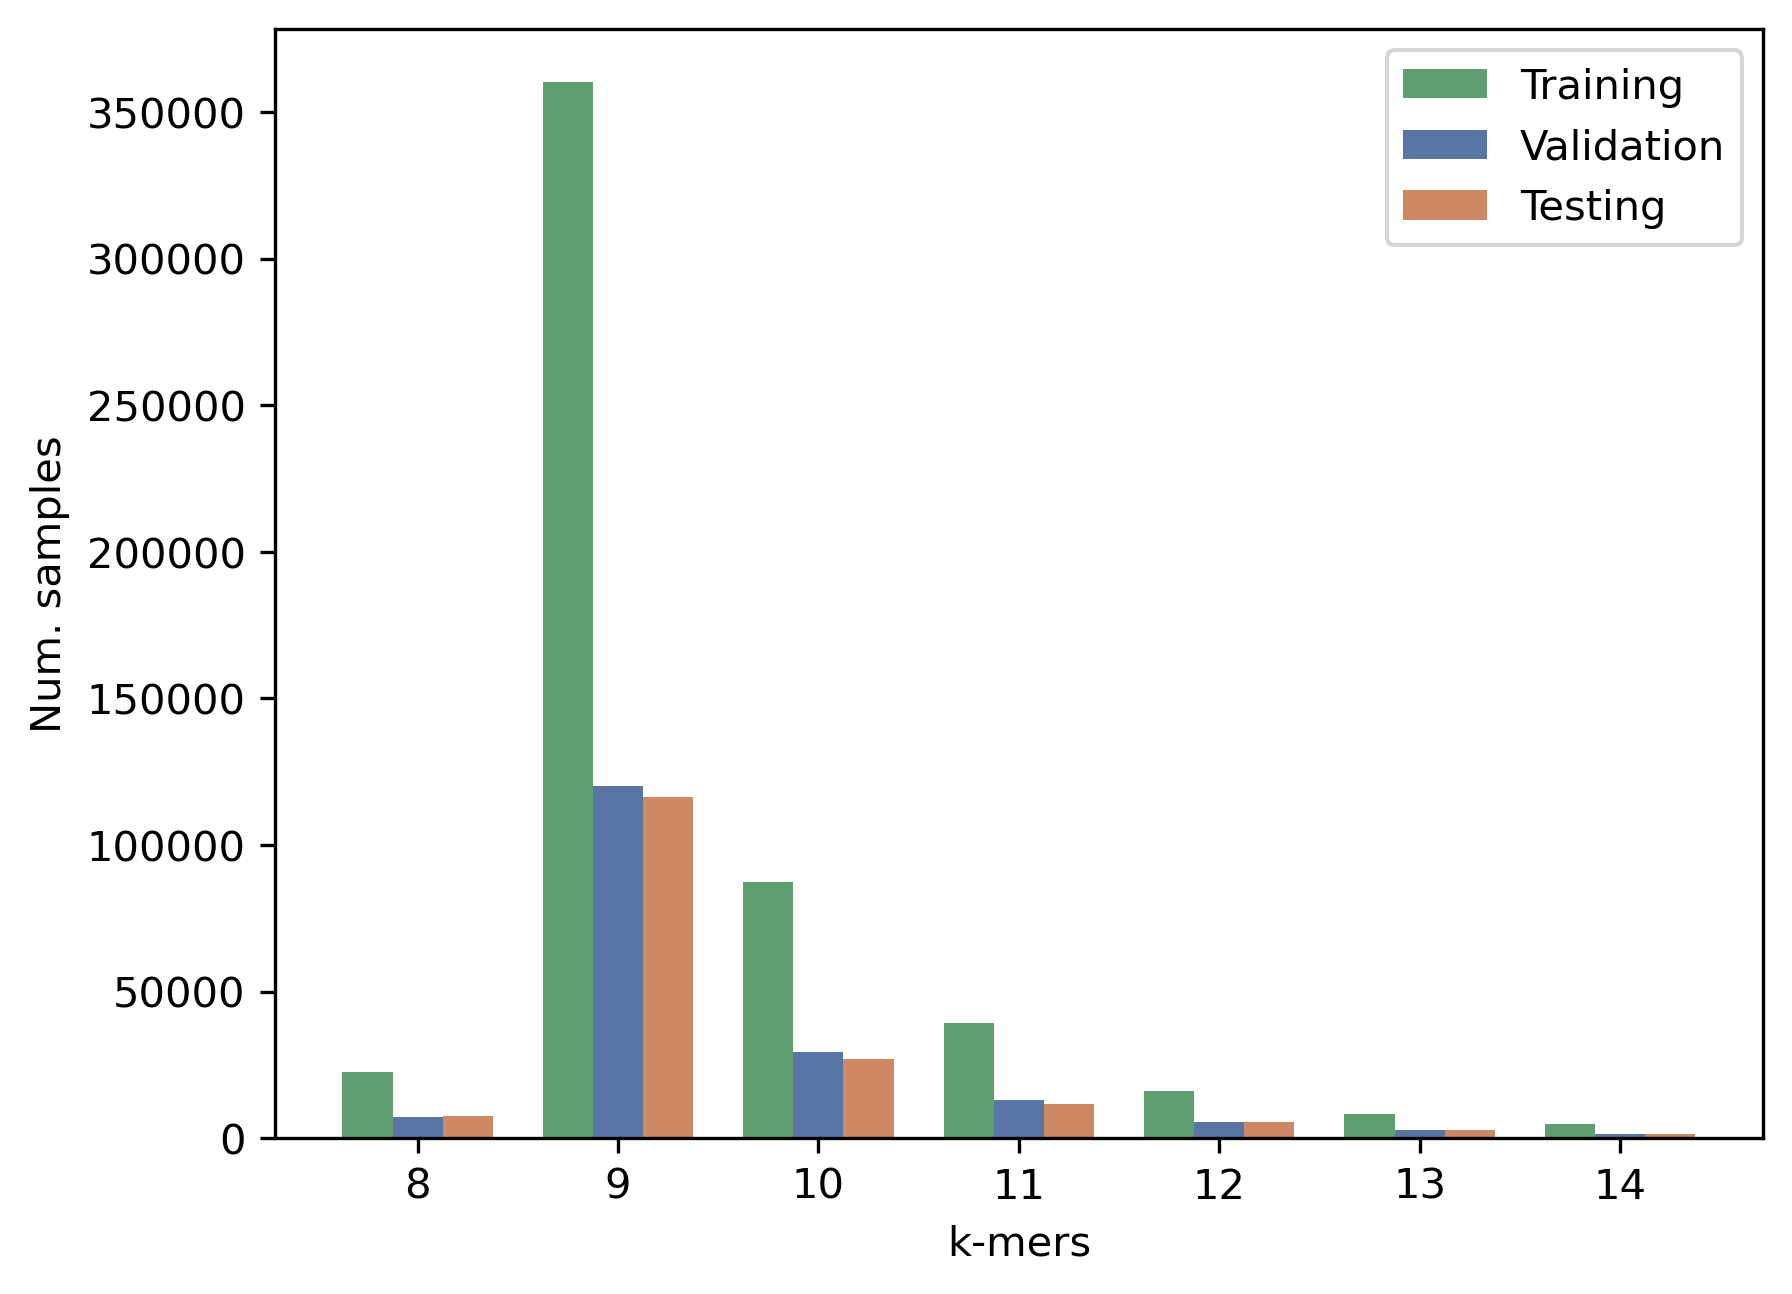
\includegraphics[width=0.8\textwidth]{../img/proposal/dataset_samples}
	\caption{
		Cuantificación de las muestras por \textit{k-mers} dentro de los conjuntos de entrenamiento, validación y pruebas. El conjunto de datos se obtuvo de Anthem \citep{mei2021anthem}.}
	\label{fig:samples}
\end{figure}



\begin{table}[H]
	\caption[Ejemplo de algunas muestras de la base de datos]{Ejemplo de algunas muestras de la base de datos. Cada MHC es representado por una pseudosecuencia procesadas por NetMHCpan4.1. Luego los péptidos son cadenas de aminoácidos entreo 8 a 14 amino ácidos. La clase o etiqueta es un cero si existe una unión entre el péptido y el MHC o cero en caso contrario.}
	\label{tab:db_samples}
	\scriptsize
	\setlength{\tabcolsep}{0.5em} % for the horizontal padding
	{\renewcommand{\arraystretch}{1.5}% for the vertical padding
		\begin{tabular}{llll}
			%\hline
			\textbf{MHC}         & \textbf{Pseudosecuencia del MHC}                & \textbf{Péptido}        & \textbf{Clase} \\ \hline
			HLA-A*01:01 & YFAMYQENMAHTDANTLYIIYRDYTWVARVYRGY & LFGRDLSY       & 1     \\
			HLA-A*01:01 & YFAMYQENMAHTDANTLYIIYRDYTWVARVYRGY & TDKKTHLY       & 1     \\
			HLA-A*01:01 & YFAMYQENMAHTDANTLYIIYRDYTWVARVYRGY & RSDTPLIY       & 1     \\
			HLA-A*01:01 & YFAMYQENMAHTDANTLYIIYRDYTWVARVYRGY & NSDLVQKY       & 1     \\
			HLA-A*01:01 & YFAMYQENMAHTDANTLYIIYRDYTWVARVYRGY & LSDLLDWK       & 1     \\
			HLA-A*01:01 & YFAMYQENMAHTDANTLYIIYRDYTWVARVYRGY & LLQNDGFF       & 1     \\
			HLA-A*01:01 & YFAMYQENMAHTDANTLYIIYRDYTWVARVYRGY & DSDMQTLV       & 1     \\
			HLA-A*01:01 & YFAMYQENMAHTDANTLYIIYRDYTWVARVYRGY & TDYHVRVY       & 1     \\
			HLA-A*01:01 & YFAMYQENMAHTDANTLYIIYRDYTWVARVYRGY & VLDSEGYL       & 1     \\
			HLA-A*01:01 & YFAMYQENMAHTDANTLYIIYRDYTWVARVYRGY & SDFHNNRY       & 1     \\
			HLA-C*06:02 & YDSGYREKYRQADVNKLYLWYDSYTWAEWAYTWY & FDGRVVTRSYLEKQ & 0     \\
			HLA-C*06:02 & YDSGYREKYRQADVNKLYLWYDSYTWAEWAYTWY & KPCCPDIDIFVDGK & 0     \\
			HLA-C*06:02 & YDSGYREKYRQADVNKLYLWYDSYTWAEWAYTWY & QDLKDFMRQAGEVT & 0     \\
			HLA-C*06:02 & YDSGYREKYRQADVNKLYLWYDSYTWAEWAYTWY & EGYPKSKKQFFEEV & 0     \\
			HLA-C*06:02 & YDSGYREKYRQADVNKLYLWYDSYTWAEWAYTWY & GNHISALKRRYTRR & 0     \\
			HLA-C*06:02 & YDSGYREKYRQADVNKLYLWYDSYTWAEWAYTWY & RHLRTHTGEKPYVC & 0     \\
			HLA-C*06:02 & YDSGYREKYRQADVNKLYLWYDSYTWAEWAYTWY & RGLNGGITPLNSIS & 0     \\
			HLA-C*06:02 & YDSGYREKYRQADVNKLYLWYDSYTWAEWAYTWY & SDFALKNPFYSLEM & 0     \\
			HLA-C*06:02 & YDSGYREKYRQADVNKLYLWYDSYTWAEWAYTWY & ALDSGDASPGTWSG & 0     \\
			HLA-C*06:02 & YDSGYREKYRQADVNKLYLWYDSYTWAEWAYTWY & QLVLYMKAAQLLAA & 0    \\ %\hline
	\end{tabular}}
\end{table}



\section{Clasificación binaria y Métricas}

El problema de predicción de unión pMHC es un problema de regresión. Sin embargo, basado en el conjunto de datos utilizado en este estudio, también podría abordarse como un problema de clasificación binaria al seleccionar un umbral apropiado. Las métricas de aprendizaje automático utilizadas en este trabajo son: \textit{accuracy, precision, recall, f-1 score, Area Under the Curve (AUC)}, y \textit{Matthews Correlation Coefficient} (MCC). Todas las métricas están descritas en las ecuaciones siguientes.

\begin{equation}\label{equa:acc}
	Accuracy = \frac{TP+TN}{TP+TN+FP+FN}
\end{equation}

\begin{equation}\label{equa:precision}
	Precision = \frac{TP}{TP+FP}
\end{equation}

\begin{equation}\label{equa:recall}
	Sensitivity = Recall = \frac{TP}{TP+FN}
\end{equation}

\begin{equation}\label{equa:f1}
	F1 = \frac{2*Precision*Recall}{Precision+Recall} = \frac{2 \times TP}{2*TP+FP+FN}
\end{equation}


\begin{equation}\label{equa:FPR}
	Specificity = \frac{TN}{FP+TN}
\end{equation}

\begin{equation}\label{equa:MCC}
	MCC = \frac{TP \times TN - FP \times FN}{ \sqrt{ (TP+FP)(TP  + FN)(TN+FP)(TN+FN)}  }
\end{equation}

donde \textit{TP}, hace referencia a la cantidad de muestras que eran verdaderas y han sido reconocidas como verdaderas; \textit{TN}, hace referencia a la cantidad de muestras que eran verdaderas y han sido reconocidas como falsas; \textit{FP}, son las muestras que eran falsas, pero fueron reconocidas como verdaderas; \textit{FN}, son las muestras que eran falsas y fueron reconocidas como falsas.
